\documentclass[10pt]{article}
\usepackage[margin=1in]{geometry}
\usepackage[T1]{fontenc}
\usepackage{lmodern}
\usepackage{graphicx}
\usepackage{xcolor}
\usepackage{enumitem}
\setlength{\parindent}{0pt}
\setlength{\parskip}{5pt}
\newcommand{\old}[1]{\textcolor{red}{#1}}
\newcommand{\new}[1]{\textcolor{blue}{#1}}
\pagestyle{empty}

\begin{document}

{\large\textbf{Changes made in response to your comments of 19 September}}

This page lists each comment and what changed. The last page shows the edited text with every change
marked: \old{red = removed}, \new{blue = added}. Only the abstract and the first paragraph of the
Introduction changed, so only those are shown. The body is still four pages and no number changed.

\begin{enumerate}[leftmargin=*, itemsep=5pt]

\item \textbf{The abstract's opening list reads as the only things a light curve encodes.}\\
Now: ``TESS light curves encode a star's pulsation, rotation, binarity and oscillations,
\new{among other physical properties,} but the survey produces far more light curves than can be
labelled by hand.''

\item \textbf{Say exactly which parameters we work on.}\\
Was: ``\ldots on ten tasks \old{spanning variability, asteroseismology and rotation}.''\\
Now: ``\ldots on ten tasks: \new{five variability classes, four asteroseismic targets and rotation
period}.''\\
The full list of ten did not fit in the four-page limit; it is in Table~1. One nuance: pre-training
uses no labels, so these are the quantities we \emph{evaluate} on, not train on.

\item \textbf{``Why do we care'' about those quantities is never set up.}\\
Not changed in this version. The four-page limit leaves room for one clause in the Introduction (``and
with them its age, interior and companions''). A motivation paragraph is on the list for the arXiv
version.

\item \textbf{Cadence language is too fixed (full-frame images are now 200\,s).}\\
Was: ``full-frame images, \old{every 30 or 10 minutes}, for every star in the field''.\\
Now: ``full-frame images of every star in the field \new{at cadences that change between mission
cycles (30 minutes, then 10, now 200 seconds)}''.

\item \textbf{TESS does not trade sampling rate for sky coverage; it trades spatial resolution.}\\
The sentence was wrong as written and is removed. I had meant that, within TESS, only pre-selected
targets get 2-minute data; it read as a TESS-versus-Kepler claim.\\
Was: ``TESS \old{trades sampling rate against sky coverage:} 2-minute (or 20-second) light curves
for\ldots''\\
Now: ``TESS \new{returns} 2-minute or 20-second light curves for\ldots''\\
The pixel-scale and contamination point is not in this version (it needs a citation and space). It is
on the arXiv list, where it also bears on label noise in our catalogue cross-matches.

\item \textbf{``LSST will widen the gap'' --- which gap?}\\
Was: ``LSST \old{will widen the gap}.''\\
Now, with your wording: ``LSST \new{will add \emph{billions} more light curves, albeit at a cadence
of days}.''

\item \textbf{Figure 1: hard to tell which two points belong to which row.}\\
Alternate rows are now shaded, a faint dotted line runs through each row, and the two points of each
row sit closer together, so each pair traces back to its task label.

The two versions are on the next page.

\end{enumerate}

\textbf{Small trims made only to hold the four-page limit} (each of the edits above added a line):
``features from \old{these light curves}\new{them}'' in the abstract; ``Wide-field \old{photometric}
surveys'' and ``a cheap readout for each \old{downstream} task'' in the Introduction; ``\old{A
self-supervised}\new{An} encoder here therefore has to be chosen by a held-out probe'' in the
Discussion (not shown on the last page).

\newpage
\textbf{Figure 1, before and after}

\textit{Before}\par
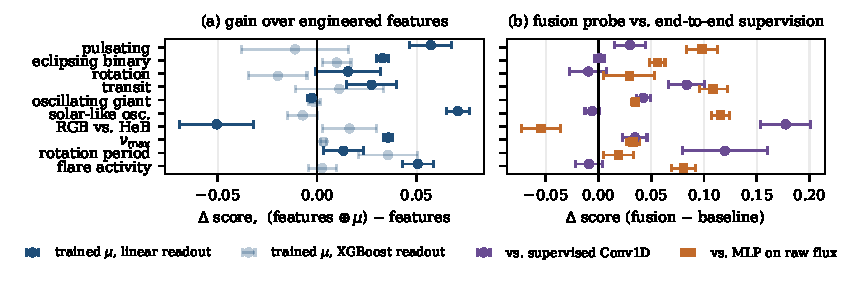
\includegraphics[width=0.92\linewidth]{fig1_before.pdf}

\textit{After}\par
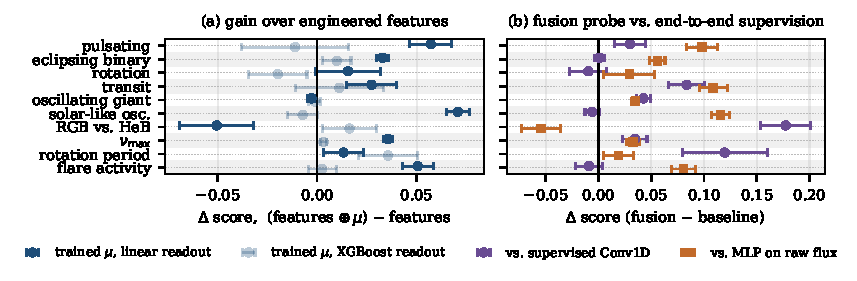
\includegraphics[width=0.92\linewidth]{fig1_after.pdf}

\end{document}
